\documentclass{homework}

\title{Problem Set 5}
\author{Kevin Evans}
\studentid{11571810}
\date{October 7, 2020}
\setclass{Physics}{443}
\usepackage{amssymb}
\usepackage{mathtools}

\usepackage{amsthm}
\usepackage{amsmath}
\usepackage{slashed}
\usepackage{relsize}
\usepackage{threeparttable}
\usepackage{float}
\usepackage{booktabs}
\usepackage{boldline}
\usepackage{changepage}
\usepackage{physics}
\usepackage[inter-unit-product =\cdot]{siunitx}
\usepackage{setspace}

\usepackage[makeroom]{cancel}
%\usepackage{pgfplots}

\usepackage{enumitem}
\usepackage{times}

\usepackage{tcolorbox}

\begin{document}
	\maketitle
	\begin{enumerate}
		\item \begin{enumerate}
			\item The systems matrix can be characterized as $\bvec{R}_2 \bvec{T} \bvec{R}_1$, \begin{align*}
				\bvec{S} & = \begin{pmatrix}
					1 & 0 \\
					\lim\limits_{r \to \infty} \frac{n - 1}{r} & n
				\end{pmatrix}
				\begin{pmatrix}
					1 & d \\
					0 & 1
				\end{pmatrix}
				\begin{pmatrix}
					1 & 0 \\
					\frac{ 1 - n }{n R} & \frac{1}{n}
				\end{pmatrix} \\
				& = \begin{pmatrix}
					1 & 0 \\
					0 & n
				\end{pmatrix}
				\begin{pmatrix}
					1 + \frac{d(1 - n)}{nR} & \frac{d}{n} \\
					\frac{1 - n}{nR} & \frac{1}{n} 
				\end{pmatrix} \\
				& = \begin{pmatrix}
					1 + \frac{d(1 - n)}{nR} & \frac{d}{n} \\
					\frac{1 - n}{R} & 1
				\end{pmatrix}
			\end{align*}
		
			\item At the thin lens limit $d \to 0$, the systems matrix becomes \begin{align*}
				\bvec{S} & = \begin{pmatrix}
					1 & 0 \\
					\frac{1-n}{R} & 1
				\end{pmatrix}
				\intertext{From inspection of the systems matrix, the focal length is}
				f & = \frac{R}{n - 1}
			\end{align*}
		\end{enumerate} 
	
		\item Hecht 5.26.
			Assuming a thin lens, the systems matrix will be \begin{align*}
				\bvec{S} & = \begin{pmatrix}
					1 & 0 \\
					\frac{n_2 - n_1}{n_1} \left(\frac{1}{R_2} - \frac{1}{R_1}\right) & 1
				\end{pmatrix} \\
				& = \begin{pmatrix}
					1 & 0 \\
					\frac{2(n_2 - n_1)}{n_1 R} & 1
				\end{pmatrix} \\
				f & = \frac{n_1 R}{2(n_2 - n_1)}
				\intertext{For $n_2 = 1.5$ and $R=\SI{12.5}{\centi\meter}$,}
				f & = -\frac{\SI{12.5}{\centi\meter}}{2(1.5 - 1)} \\
					& = -\SI{12.5}{\centi\meter} \\
				\intertext{For $n_1 = 1.628$,}
				f & = -\frac{1.628 \left(\SI{12.5}{\centi\meter}\right)}{2(1.5 - 1.628)} \\
					& = \SI{79.5}{\centi\meter}
			\end{align*}
		
		\pagebreak
		
		\item Hecht 5.47. Using the thin lens equation, $s_{i1} = \infty$, as the object is at the first lens' focal point. \begin{align*}
			\frac{1}{f_2} & = \frac{1}{s_{o2}} + \frac{1}{s_{i2}} \\
			s_{i2} & = f_2 = \SI{-20}{\centi\meter} \text{\quad (rel. to $L_2$)}
		\end{align*}
		Since the image from the first lens is at $+\infty$, it will be at $-\infty$ relative to the second lens, and the total transverse magnification will have a positive sign, \begin{align*}
			M_T & = M_{T1} M_{T2} = \frac{\cancel{s_{i1}}}{s_{o1}} \frac{s_{i2}}{\cancel{s_{o2}}} \\
				& = \frac{20}{30} = 0.667
		\end{align*}
		\begin{center}
			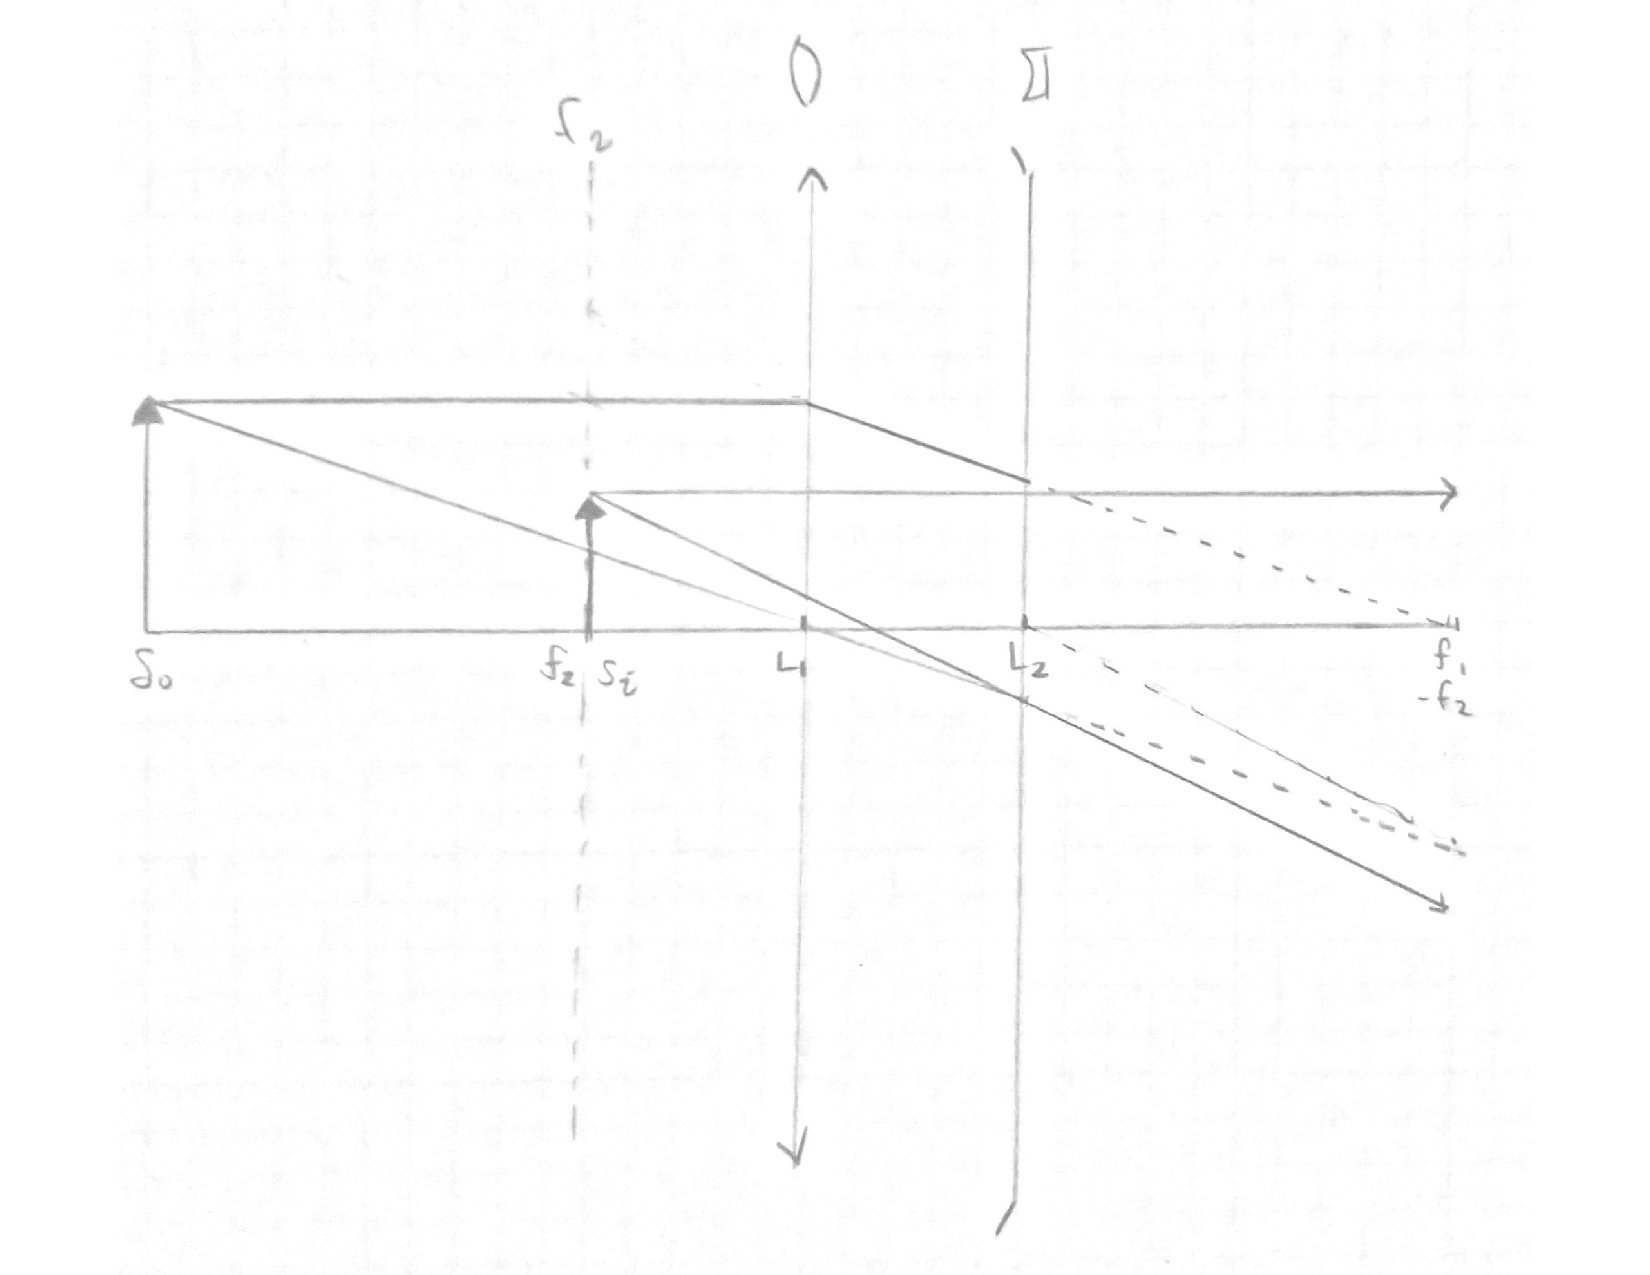
\includegraphics[width=0.9\linewidth]{Scanned_20201005-1407.pdf}
		\end{center}

		\item \begin{enumerate}
			\item% TODO, fix this, only for theta c, not theta i. want theta na? no, want derive rln for min angle for tir. 
			The critical angle within the fiber is \begin{align*}
				\theta_c & = \sin[-1]( 1.46 / 1.6) = 65.9^\circ
			\end{align*}
		
			\item From (5.61), \begin{align*}
				\mathrm{NA} & = \left(n_f^2 - n_c^2\right)^{1/2} \\
					& = (1.6^2 - 1.46^2)^{1/2} \\
					& = 0.655
			\end{align*}
		\end{enumerate}		
	\end{enumerate}
\end{document}